\chapter{How to Show, Not Tell}

This lecture has almost no mathematics in the ordinary sense, but it does have a formal backbone. We are asked to think of prose as an inferential system. Do we hand the reader the conclusion, or do we hand the reader the evidence from which the conclusion may be recovered? The lecture unfolds with considerable care: a deliberately bad opening passage creates the problem, a series of concessions prevents us from turning the lesson into a slogan, and six principles then sharpen the craft. We will follow that order, because the argument depends as much on its progression as on its individual claims.

\begin{remark}
There is no literal board mathematics to transcribe here. The displayed equations below are editorial schemata: they compactify the lecture's logic, but they are not meant to suggest that a symbolic formalism appeared on screen.
\end{remark}

\section{The Opening Failure}

The lecture does not begin with a definition. It begins with a failure. We are given a wilderness passage in which a girl is said to be afraid, the sounds are said to be frightening, and the ground is said to feel like a guardian. Everything important is announced. Very little is made palpable.

That is the correct pedagogical opening. The lecturer wants us to feel the weakness before we are told its name. The prose names fear without dramatizing it, and names atmosphere without creating it. We are given emotional verdicts without the sensory or narrative pressure that would justify them.

\subsection{Question \& Answer}

The lecture stops and asks the question that governs the whole chapter.

What is wrong with this picture?

What is wrong is not that the passage contains emotion words. The trouble is that the passage has supplied its conclusions before it has supplied its evidence. Fear is asserted, not enacted. Safety is asserted, not earned. The reader is told what to think and feel at precisely the point where the scene ought to be making those feelings unavoidable.

\begin{definition}
In the sense of this lecture, \emph{telling} states a conclusion, summary, trait, or emotion directly, whereas \emph{showing} furnishes the dramatic, sensory, behavioral, or perspectival evidence from which the same conclusion may be inferred.
\end{definition}

K.\ M.\ Weiland's compact distinction gives the lecture its first clean axis:
\begin{align}
\text{showing} &= \text{dramatizing},\\
\text{telling} &= \text{summarizing}.
\end{align}

That is already a correction to a common confusion. Summary is not the enemy. Unsupported summary is the enemy. The lecture will spend the rest of its time telling us when a summary is doing useful work, and when it is prematurely closing the scene.

\section{Showing, Telling, and the Reader's Work}

Having posed the problem sharply, the lecture immediately softens the rule. Telling is not inherently bad. If we tried to show every passing fact, every interval of time, every routine motion, our fiction would become swollen and shapeless. Stories need compression. They need bridges. They need broad sweeps as well as fully inhabited moments.

That is why the Secret Garden example appears here. We are told that Mary Lennox is a disagreeable-looking child who has often been ill, but the prose does not stop with the verdict. It moves at once to the thin face, the thin body, the light hair, the sour expression. The summary is anchored in proof. That is the lecture's model of a legitimate blend.

The lecture's central logic may be written schematically as
\begin{equation}
\text{concrete detail} \leadsto \text{reader inference} \leadsto \text{emotion or judgment}.
\end{equation}

This is the point at which Andrew Stanton's storytelling metaphor becomes useful. The transcript is slightly garbled, but the secure idea is plain. We should not give the audience ``4'' when what we want is active participation. We should give them ``2+2'' and let them perform the last step for themselves:
\begin{equation}
2+2 \to \text{audience inference}, \qquad 4 \to \text{premature closure}.
\end{equation}

The lecture insists that this is not decorative advice. Readers want to work, provided the work is artfully hidden inside the experience. They want to deduce, complete, and discover. In that sense, showing is a discipline of organized incompleteness: we omit the final label so that the reader may arrive there under pressure of the scene.

\begin{figure}[h]
\centering
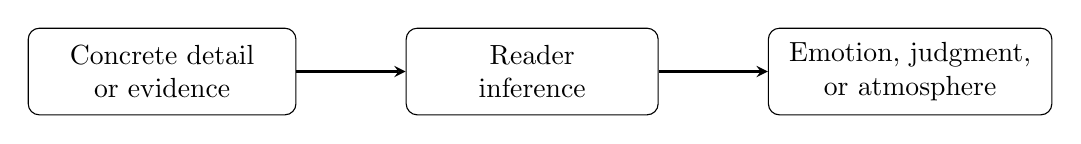
\begin{tikzpicture}[>=stealth]
\node[draw, rectangle, rounded corners, minimum width=3.4cm, minimum height=1.1cm, align=center] (a) at (0,0) {Concrete detail\\or evidence};
\node[draw, rectangle, rounded corners, minimum width=3.2cm, minimum height=1.1cm, align=center] (b) at (4.7,0) {Reader\\inference};
\node[draw, rectangle, rounded corners, minimum width=3.6cm, minimum height=1.1cm, align=center] (c) at (9.5,0) {Emotion, judgment,\\or atmosphere};
\draw[->, thick] (a) -- (b);
\draw[->, thick] (b) -- (c);
\end{tikzpicture}
\caption{The lecture's basic inferential pipeline. We do not begin by naming the verdict; we begin by supplying the evidence from which the verdict becomes almost inevitable.}
\end{figure}

From here the lecture broadens its claim. What is true of cinematic storytelling is also true of prose. The reader cares more when the meaning is implied than when it is pointed out. That is why the lecture can now step back and ask where this mantra came from.

\section{Why the Mantra Exists}

Before turning to the six principles, the lecture inserts a brief historical detour. This is not ornamental. It explains why the rule has the force it does.

The lecturer places the modern slogan in the tradition of realism: the attempt to render ordinary life with enough immediacy and honesty that it no longer feels romanticized or rhetorically overmanaged. Percy Lubbock is then brought in as a major formalizer of the distinction. His key thought is that fiction becomes art when the story is treated as something to be shown, so that it seems to tell itself.

Janice Hardy's practical restatement translates that literary history back into workshop language. As long as the line feels like the character's thought, perception, or pressure, we are generally safe. When it sounds like the author stepping in to decode the scene, immersion weakens.

We may summarize the practical tendency this way:
\begin{equation}
\text{authorial explanation} \downarrow \;\Longrightarrow\; \text{reader immersion} \uparrow.
\end{equation}

This is not an absolute law; the lecture will later restore exposition and narration to their proper place. But the detour clarifies the real target. The problem is not that telling exists. The problem is that the author becomes too visible at the very point where we want the reader to live the scene from within.

With that larger motivation in place, the lecture is ready to become practical. It now turns, in order, to six guiding principles.

\section{Evidence, Concrete Detail, and Sensory Specificity}

The first three principles form a natural cluster. They all answer the same question from different angles: if we do not simply assert the emotional or descriptive conclusion, what do we put in its place?

\subsection{Evidence Before Verdict}

The first move is the cleanest. If a narrator says that a husband is kind-hearted, if a protagonist believes a friend is guilty, or if a line says that Adam knew Gwen liked him, the lecturer asks us to pause before the conclusion and look for its ground. What led anyone to think this?

A thought-verb exercise cited in the lecture makes the same point. For revision purposes, we temporarily distrust verbs such as \emph{knew}, \emph{believed}, \emph{wanted}, \emph{realized}, and \emph{imagined}. Not because they are forbidden, but because they often hide the real scene.

\paragraph{Worked revision.} The lecture's sample line is ``Adam knew Gwen liked him.'' The repair is not mysterious; it is methodical.
\begin{enumerate}
\item Start with the conclusion: Adam knew Gwen liked him.
\item Ask what Adam actually perceives.
\item Replace the hidden judgment with repeated locker encounters, the heel mark on the painted metal, the smell of perfume, and the warm combination lock.
\item Stop when the reader can reach Adam's conclusion unaided.
\end{enumerate}

In schematic form,
\begin{align}
\text{``Adam knew Gwen liked him''}
&\xrightarrow{\text{revision}}
\text{locker} + \text{heel mark} + \text{perfume} + \text{warm lock}.
\end{align}

So the first principle is not merely ``add detail.'' It is more exact: replace the conclusion with the evidence that licenses the conclusion.

\subsection{From the Abstract to the Concrete}

The second principle takes the same logic and applies it to emotion words and evaluative adjectives. Harvey Chapman's example does the job efficiently. Instead of saying that Toby walked home happier than he had ever felt, the better version gives us the grin that will not leave his face and the buoyant, almost stumbling energy of his movement.

This may be written as a general revision rule:
\begin{equation}
\text{abstract label} \xrightarrow{\text{revision}} \text{observable evidence}.
\end{equation}

A few of the lecture's substitutions show the pattern:
\begin{align}
\text{happy}
&\xrightarrow{\text{showing}}
\text{goofy grin} + \text{springing movement},\\
\text{eerie}
&\xrightarrow{\text{showing}}
\text{a forest humming with the cries of children long dead}.
\end{align}

The point is not that abstraction is always illegitimate. The point is that abstract words often arrive too soon. They tell us what the scene means before the scene has made meaning felt. The lecture's eerie-forest example is useful for precisely this reason. ``The dark forest felt eerie'' is not false. It is simply weak. The revised line does not argue against the adjective; it earns it.

\subsection{Question \& Answer}

How do we know that we are still writing in abstraction?

The lecture's operational answer is simple: ask whether the camera can see it. That is not a complete test, because prose can also invoke smell, touch, taste, and sound. But it is a strong first filter. If the camera cannot see it, we should ask what sensory evidence, if any, has actually been supplied.

This leads directly to a third schematic rule:
\begin{equation}
\text{cause statement} \xrightarrow{\text{showing}} \text{visible or sensory effect}.
\end{equation}

Jerry Jenkins's examples are ideal here:
\begin{align}
\text{cold}
&\xrightarrow{\text{showing}}
\text{collar up} + \text{scarf tightened} + \text{hands in pockets} + \text{face turned from wind},\\
\text{blindness}
&\xrightarrow{\text{showing}}
\text{white cane feeling for the bench},\\
\text{late fall}
&\xrightarrow{\text{showing}}
\text{leaves crunching underfoot}.
\end{align}

This is one of the lecture's most important local derivations. Instead of naming the cause, we write its trace. Instead of ``it was cold,'' we show what cold does. Instead of ``it was late fall,'' we let the ground sound the season for us.

The lecture then extends the point beyond visibility. Delilah Dawson's market scene becomes stronger not merely because it is concrete, but because it becomes sensorily and locally concrete: cinnamon, coffee, silken tassels, powdered saffron. A scene becomes more immersive when its particulars are both vivid and singular to its world.

Finally, the lecturer adds a subtle warning. Even a technically visual scene may be inert if its details are too expected. A rainy funeral may be clear, and yet stale. That is why the lecture pauses over Gail Carson Levine's advice: if the scene feels clich\'ed, change the setting, change the emotional angle, or introduce one local anomaly that breaks expectation. At this stage we are no longer merely replacing abstraction with detail; we are replacing generic detail with detail that belongs to \emph{this} story.

\section{Beyond Stock Body Language}

At this point the lecture makes an important correction. Once writers are told to show, they often reach for the quickest available shorthand: clenched fists, crossed arms, gritted teeth, racing hearts, rolling stomachs. These are not useless, but they are very easy to overuse.

The danger is now more precise than before. Earlier, the danger was bare abstraction. Here the danger is a shallow concreteness: a visible sign that signals some emotional charge, but does not tell us enough about its source.

\subsection{Question \& Answer}

Is body language enough?

Usually not. It may indicate that \emph{something} is happening, but it often fails to communicate \emph{what kind} of thing is happening. Anger may resemble frustration, humiliation, jealousy, panic, or grief when reduced to a single stock gesture. The lecture's point is that body language is often too compressed to carry emotional nuance on its own.

Robin Patchen's before-and-after example makes this decisive. In the first version, Mary sees the clock, her heart nearly leaps out of her chest, her stomach rolls, and she fears that something is wrong. At first glance, this looks like showing, because we do see bodily reaction. But the lecturer insists that the scene still feels melodramatic and overexplained. The body is doing all the work; the thought-process is barely there.

The revised version changes the center of gravity. Sunlight streams through the window. Mary wakes rested. She sees the clock. She realizes that little Jane has slept through the night. Then another memory enters: Billy. Action follows almost at once: she flips the covers back, snatches the robe, repeats the doctor's reassurance to herself. Now the emotion has a contour. It is not just alarm; it is alarm under the pressure of memory and denial.

The lecture compresses this into a causal chain worth preserving:
\begin{equation}
\text{thoughts} \to \text{emotions} \to \text{actions}.
\end{equation}

This is perhaps the lecture's cleanest ``equation.'' It tells us where to look when a scene feels emotionally thin. If we leap too quickly to bodily shorthand, we skip the thought that gives the feeling its exact shape. If we restore the thought, the resulting action becomes more particular and more credible.

A useful revision sequence is therefore:
\begin{enumerate}
\item Replace generic visceral alarm with the local sequence of perception, recognition, and memory.
\item Let the setting participate: the open window, the sunlight, the clock, the robe.
\item Let verbs carry force: \emph{flipped} and \emph{snatched} are stronger than neutral motion verbs.
\item Let sentence structure itself help; short units and abrupt pivots can perform urgency.
\end{enumerate}

The lecture then turns this into practical advice. When the scene is highly emotional, we should often slow it down. Let us hear the character's thought. Let a few details stand. Let the action arise. Readers are intelligent enough to reconstruct the emotion if the thoughts and actions are truly there.

\section{Dialogue, Telegraphing, and Redundancy}

The fifth principle transfers the same discipline into speech. Dialogue can show emotion directly, provided we trust the words and the scene to do the work.

The lecture begins with an obvious case. If Mary is angry at Bob, the line itself can carry the anger. Once the words already perform the feeling, the tag ``angrily'' tends to weaken rather than help. It tells us what the line has already shown.

\subsection{Question \& Answer}

When does dialogue start telegraphing instead of showing?

Dialogue begins telegraphing when narration announces a motive, intention, or tonal conclusion that is already present in the exchange itself. If we write that he tried to be diplomatic, and then give him a conciliatory line, we have doubled the information. If we write that she changed the subject, and then immediately have her move the conversation elsewhere, we have explained what the reader could already infer.

In schematic form,
\begin{align}
\text{dialogue} + \text{redundant explanation}
&\to \text{telegraphing},\\
\text{dialogue} + \text{precise action beat}
&\to \text{sharper subtext}.
\end{align}

The revised dialogue in the lecture obeys this rule. Instead of explanatory narration, it gives a selective beat and a selective tag: he pinches the bridge of his nose; she whispers. The line itself continues to carry the main force, but the surrounding detail sharpens the social geometry without decoding it for us.

The lecture then pushes the point one step further. If we want to strengthen emotional dialogue, it can help to draft the scene almost as if it were a play. That constraint forces us to carry tone in the exchange itself. Oscar Wilde is invoked precisely because his dialogue can do this. A clipped objection, an incredulous repetition, a small turn of phrase: all of these can make a feeling audible before narration explains it.

This prepares the transition into the final principle. If we can trust dialogue more, we can also trust point of view more broadly. The same issue of redundancy returns in exposition and description.

\section{Narrative Voice, Exposition, and Pacing}

The sixth principle broadens the lecture from local repair to narrative architecture. Showing is not only a matter of replacing one adjective with one image. It is also a matter of point of view, exposition, and pace.

The lecture begins from a small set of paired examples. ``He was rude and inconsiderate'' becomes a line shouted at a woman struggling with a stroller. ``She was uncomfortable around him'' becomes ``She stiffened in his embrace.'' ``The house was huge'' becomes a kitchen large enough to house the whole family. ``She was hungry'' becomes a bowl of soup nearly inhaled. These are stronger not merely because they are concrete. They are stronger because they are perspectival. Each line arrives from a mind placed inside a situation.

That same principle controls exposition. Janice Hardy's distinction between the reader's benefit and the character's benefit is crucial. Information that exists only to brief the audience often sounds external to the scene. Information filtered through what the character would notice, fear, ask, or say remains inside the story's field of experience.

The restaurant example sharpens this insight. Rain, pancakes, an envelope, a ticking clock: the external facts need not change very much. But once the point of view changes, the whole scene changes. For a military mind, the rain becomes gunfire. For a frightened girl, the window becomes blur and enclosure. This is not a cosmetic difference. It is narrative voice doing structural work.

The same pressure explains why ``as you know Bob'' dialogue fails. When one character explains to another what they both already know, the line is not serving the characters. It is serving the reader too openly. The author has become visible again.

At this point the lecture performs its last and most important correction. The true lesson is not ``show always.'' The true lesson is ``show, don't just tell.'' Telling remains one of our pacing tools. It is what lets us bridge, compress, summarize, and move. Showing is what lets us dwell, inhabit, and intensify.

We may state the balance schematically as
\begin{equation}
\text{telling} + \text{specific detail} = \text{a strong blend when pacing requires it}.
\end{equation}

A useful further compression of the lecture's pacing rule is
\begin{align}
\text{scene importance} \uparrow &\Rightarrow \text{showing density} \uparrow,\\
\text{bridging or compression need} \uparrow &\Rightarrow \text{telling fraction} \uparrow.
\end{align}

The lecture's closing ``cheat sheet'' can be summarized as follows.

\begin{table}[h]
\centering
\begin{tabular}{|p{0.42\textwidth}|p{0.42\textwidth}|}
\hline
\textbf{Tell or blend when we need speed} & \textbf{Show when we need presence} \\
\hline
Bridges from point A to point B & Emotions \\
\hline
Routines, time passing, repeated conversations & Sensations: sight, sound, smell, taste, touch \\
\hline
Broad exposition or occasional backstory & Assumptions and judgments about people or places \\
\hline
Some world-building summaries & Dialogue tone, motive, and conversational intention \\
\hline
Large-scale thought or narrative sweep & The concrete traces from which feeling is inferred \\
\hline
\end{tabular}
\caption{The lecture's final pacing balance. Telling is not abolished; it is allocated.}
\end{table}

This is why the lecture can end, without contradiction, by praising strong narrative voice in exposition. A narrated opening may still be powerful if its voice carries tension and pressure. Telling is not expelled from fiction. It is disciplined and placed.

That final balance prepares the return to the opening wilderness example. The Delia Owens passage works because it does not merely announce that fear is gone and comfort has arrived. It lets the land catch the girl when she stumbles. It lets pain seep away like water into sand. It lets the marsh become mother. The emotional transformation is no longer reported from outside; it is enacted through image, movement, and voice. The lecture closes where it began, but the bad example has now been metabolized into a standard.

\section{Summary}

We may now state the lecture's argument in its mature form. Showing is not the refusal of telling. It is the discipline of withholding the final verdict until the scene has supplied the evidence from which that verdict emerges.

When a line feels weak, the lecture gives us a rigorous sequence of questions:
\begin{itemize}
\item Have we supplied a conclusion before we have supplied the evidence?
\item Have we named an emotion where a concrete trace would do more work?
\item Can the camera see what we have written, or can the senses at least register it?
\item Are we leaning on stock body language instead of thought, setting, and action?
\item Are we explaining dialogue that already explains itself?
\item Is exposition serving the character's point of view, or only briefing the reader?
\end{itemize}

The final principle is therefore balanced and practical. We show when we want presence, pressure, and reader participation. We tell when we need compression, transition, or broad narrative sweep. The craft lies in knowing which moments deserve ``2+2'' and which moments may honestly be given as ``4.''